\chapter{Hybridní hry}
Hybridní hry kombinují jak prvky fyzické, tak digitální. Jedná se o hry, které mají jakékoliv napojení na technologii, ať už je to elektronické bankovnictví ve hře Monopoly Super Electronic Banking, či mobilní aplikace Pokémon GO, která vás pomocí map navádí k navštívení památek a zajímavých míst. Podobná spojení vyústí ve zcela nové herní zážitky, které si hráči mohou vyzkoušet.\cite{hybrid_board_games_design}

\section{Vývoj hybridních her}
První hybridní hry se začaly formovat již na začátku 20. století, kdy se začaly objevovat první hry s elektrickými prvky. Tyto hry byly většinou jednoduché elektrické obvody, které hráč propojoval pro různé efekty. V průběhu času se tyto hry stávaly složitějšími a začaly se objevovat hry, které využívaly počítačové technologie. Hybridní hry mohou být kategorizovány do několika skupin, které se liší podle toho, jakým způsobem technologie využívají.\cite{history_of_hybrid_games}

\subsection{Stolní hry s vlastním zařízením}
Mezi takovéto hry patří již výše zmíněný Monopoly Super Electronic Banking, který obsahuje elektronické bankovnictví, nebo známá hra Operation, ve které se nesmíte dotknout kovových částí na hrací desce, jinak se rozezní siréna. 

Tato kategorie hybridních her je rozhodně nejstarší. První hrou využívající elektrického proudu, a tudíž zařazenou do hybridních her, je hra Electra (původním názvem Lichtra), kterou můžeme vidět na obrázku \ref{fig:electra}. Jedná se o jednoduchou kvízovou hru, která vyšla už v roce 1910 v Německu a byla vytvořena společností Sala Games. Hra obsahovala jednoduchý elektrický obvod, který se uzavřel, pokud hráč odpověděl správně. Po této hře následovala dlouhá éra her, jejichž elektronika také spočívala pouze v propojení jednoho, či několika málo obvodů.\cite{history_of_hybrid_games, boardgames_with_apps}

\begin{figure}[H]
    \centering
    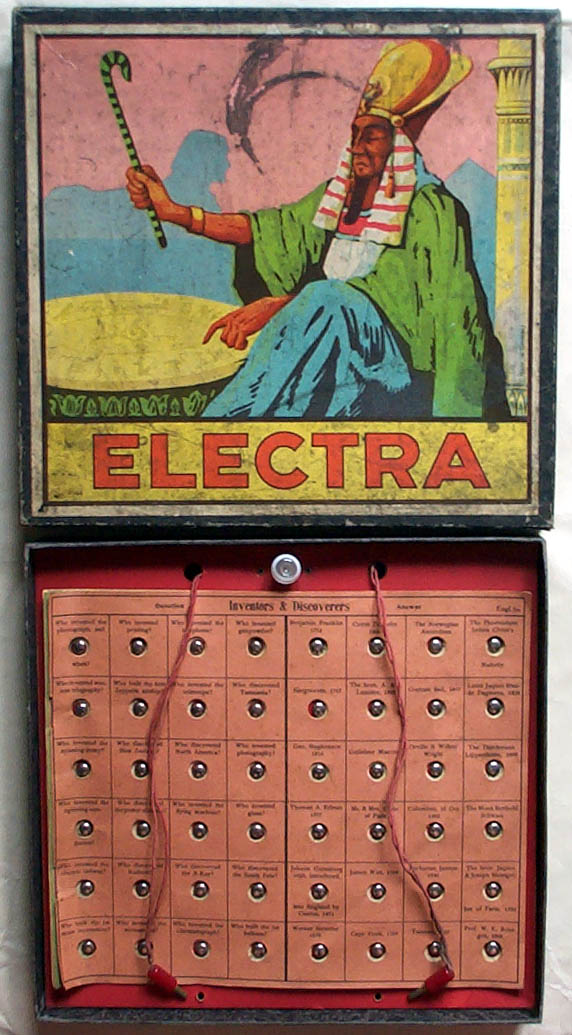
\includegraphics[width=0.3\textwidth]{resources/figures/electra.jpg}
    \caption{Hra Electra, první hybridní hra.\cite{history_of_hybrid_games}}
    \label{fig:electra}
\end{figure}

Další zmínku ve vývoji her v této kategorii si zasloužila hra Voice of the Mummy, která vyšla v roce 1971. Hra měla v herním plánu zabudovaný přehrávač, který měl simulovat hlas mumie, která při přejití určitých herních polí hráčům určovala další postup.\cite{voice_of_the_mummy}

První hrou, která ve svém designu používala počítačové zařízení byla francouzská hra Simulateur JR10, která vyšla roku 1972. Jednalo se bitevní hru, ve které hráči ovládali různé jednotky. Při střetu jednotek se do počítače vložil děrný štítek s odpovídajícími jednotkami a počítač podle naprogramovaných kritérií náhodně určil výsledek střetu.\cite{simulateur_jr10}

\subsection{Stolní hry s vlastní aplikací}
V roce 1972 vyšla herní konzole Magnavox Odyssey, která je uznávaná jako první domácí herní konzole na světě. Zároveň s ní vyšlo i několik her, které kombinovaly fyzickou hrací desku s počítačovým programem. Celé UI této konzole zahrnovalo pouze několik svítících bodů na obrazovce, proto byl ke každé hře přiložen lehce průsvitný plán s potiskem, který se na obrazovku přichytil. Součástí větsiny her byly i fyzické komponenty, které měly u hráčů sloužit k přirozenějšímu pozvolnému přechodu ze stolních her na hry digitální.\cite{magnavox_odyssey} Jednou z her na tuto konzoli byla hra Invasion. Její fyzická složka zahrnovala kostky, sadu karet, sadu tokenů a hrací desku. Samotný program byl pak určen k soubojům mezi hráči. Tyto komponenty můžeme vidět na obrázku \ref{fig:invasion}\cite{invasion,invasion_gameplay}

\begin{figure}[H]
    \centering
    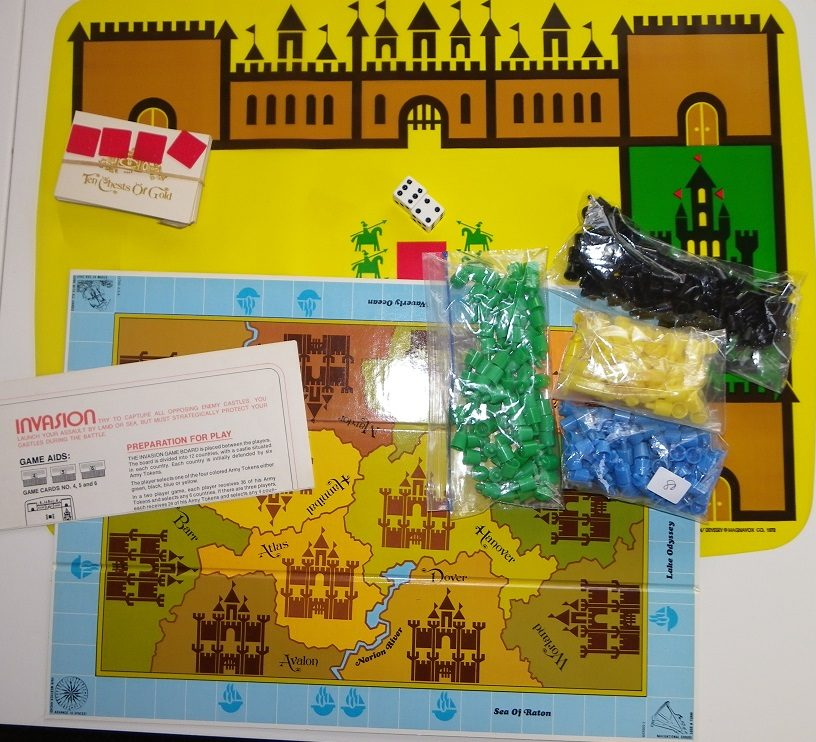
\includegraphics[width=0.45\textwidth]{resources/figures/invasion.jpg}
    \caption{Fyzické komponenty a nalepovací plán hry Invasion.\cite{invasion}}
    \label{fig:invasion}
\end{figure}

V roce 1983 vyšlo hned několik her, které kombinovaly fyzickou hrací desku s digitální hrou. Jednou z nich byla společností Epyx vydána hra Oil Barons. Jednalo se o počítačovou hru, která byla určena pro zařízení DOS, Apple II a Commodore 64. Její součástí byla fyzická hrací deska a několik herních tokenů. Samotný program měl za úkol simulovat náhodné výsledky a udržovat stav hry. UI této hry bylo jednoduché a odpovídalo své době (obrázek \ref{fig:oil_barons}).\cite{oil_barons}

\begin{figure}[H]
    \centering
    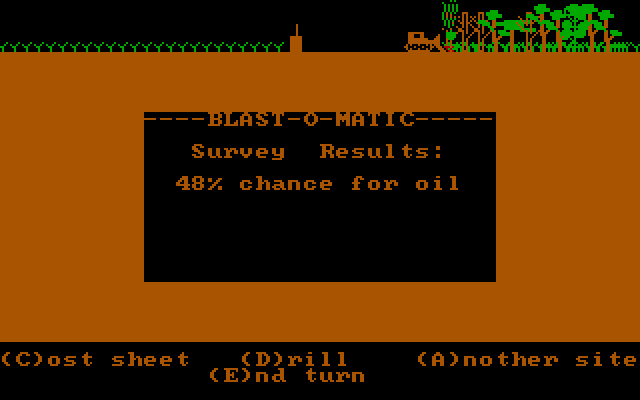
\includegraphics[width=0.45\textwidth]{resources/figures/oil_barons.png}
    \caption{Příklad GUI hry Oil Barons.\cite{oil_barons}}
    \label{fig:oil_barons}
\end{figure}

Další významný vývoj této kategorie hybridních her se uvíjel nejčastěji k mobilním aplikacím a takzvaným companion apps (podpůrným aplikacím). Tyto aplikace slouží k různým účelům, jako je například výběr, či správa herních prvků, nebo vyprávění příběhu. Většina těchto aplikací je oficiální součástí dané hry a nelze ji bez ní hrát. Mezi příklady takovýchto her patří například hra Forgotten Waters (českým názvem Na vlnách neznáma), která využívá aplikaci k vyprávění příběhu, správě nepřátel a k výběru dějové linky.

\subsection{Hry s rozšířenou realitou}
Nejmladší kategorií hybridních her jsou hry s rozšířenou realitou (AR). Tyto hry využívají technologie, které umožňují hráčům interagovat s digitálními prvky ve skutečném světě. První takovou hrou byla AR Quake, která byla vytvořena v roce 2000. Aby si hráč mohl vyzkoušet tuto hru, musel mít nasazený speciální batoh s počítačem, který pomocí gyroskopů určoval polohu hráče a promítal obraz digitálního světa přes speciální brýle. Hra byla vytvořena jako experiment, který měl ukázat možnosti AR technologií.\cite{ar_history}

Největší rozvoj v popularitě AR her nastal až s vydáním aplikace Pokémon GO v roce 2016. Tato hra využívala GPS a kameru mobilního telefonu k tomu, aby hráči mohli chodit po skutečném světě a chytat virtuální postavičky Pokémonů. Hra byla velice populární a stala se tak první AR hrou, která se dostala do povědomí široké veřejnosti.

\section{Vybrané hybridní hry}
Následující hry jsem vybral jako příklady a inspiraci pro svou práci. Jedná se o stolní hry, které nějakým způsobem využívají právě internetových aplikací pro umocnění herního zážitku, organizaci hry, či správu herních mechanismů.

\subsection{Na vlnách neznáma}
První z těchto her je Na vlnách neznáma (původním názvem Forgotten Waters), vydanou v roce 2020 společností Plaid Hat Games. Jedná se o výpravnou RPG hru ve které se hráči ujímají rolí pirátů a společně čelí dobrodružstvím a nástrahám, jenž rozmanitý příběh této hry nabízí. Hra samotná využívá oficiální internetovou aplikaci\cite{forgotten_waters_app}, která slouží k vyprávění herního děje pomocí namluvených scén a k zaznamenávání hráčských rozhodnutí, na kterých závisí dynamický rozvoj příběhu této hry. Aplikace dále udává životy a statistiky nepřátel, slouží k výběru kampaně (dějové linky) a v neposlední řadě přispívá k zážitku hráčů pomocí namluvených scén.

Fyzické komponenty hry obsahují herní plán s hexagonálními políčky a s tokeny lokací, které si hráči rozestaví podle pokynů aplikace. Dále obsahuje kartonové figurky s potiskem představující hráčské postavy a jejich osobní deník, do kterého hráč zapisuje informace o své postavě. Zároveň se ve hře nachází několik ukazatelů a počítadel, jež se využívají v několika aspektech hry. Dále je zde kniha lokací, která obsahuje popisy lokací, které se hráči mohou rozhodnout navštívit a zároveň možnosti, jež se jim v těchto lokacích nabízejí. Dále hra obsahuje balíček karet, které představují poklady a příběhové karty. Oba tyto druhy přináší hráči buďto pozitivní, nebo negativní efekty, které ovlivňují jeho postavu. Další součástí hry je sada kostek, která se využívá k určování výsledků různých akcí, jež hráči mohou provést.

\subsection{Gloomhaven}
Druhou hrou, kterou bych chtěl uvést, je Gloomhaven. Tato hra byla vydána v roce 2017 společností Cephalofair Games. Jde o kooperativní fantasy hru, ve které se hráči vcítí do role dobrodruhů, kteří se snaží přežít v nehostinném světě, plnit různé úkoly a odkrývat příběh, který před nimi leží. Hra je ve stylu dungeon crawl, což znamená, že hlavní náplní hry je postup z lokace do lokace, kde hráče čekají úkoly a boj s nepřáteli. Původně je hra koncipována jako čistě stolní hra, ale kvůli velkému množství fyzických komponentů (obrázek \ref{fig:gloomhaven_contents}), které hra obsahuje začaly vzinkat aplikace, jenž by organizaci hry usnadnily. Jednou z nich byla aplikace Gloomhaven Helper\cite{gloomhaven_helper}, která se na čas stala i oficiální aplikací pro tuto hru, avšak kvůli licenčním problémům byla tato aplikace zrušena. Po jejím stažení vzinklo několik jejích nástupců. Jedním z nich je Gloomhaven Secretariat\cite{gloomhaven_secretariat}. Tato aplikace slouží k organizaci hry, správě nepřátel i postav. Také umožňuje hráčům zaznamenávat své postupy v příběhu, výsledky bitev a další herní prvky.

\begin{figure}[H]
    \centering
    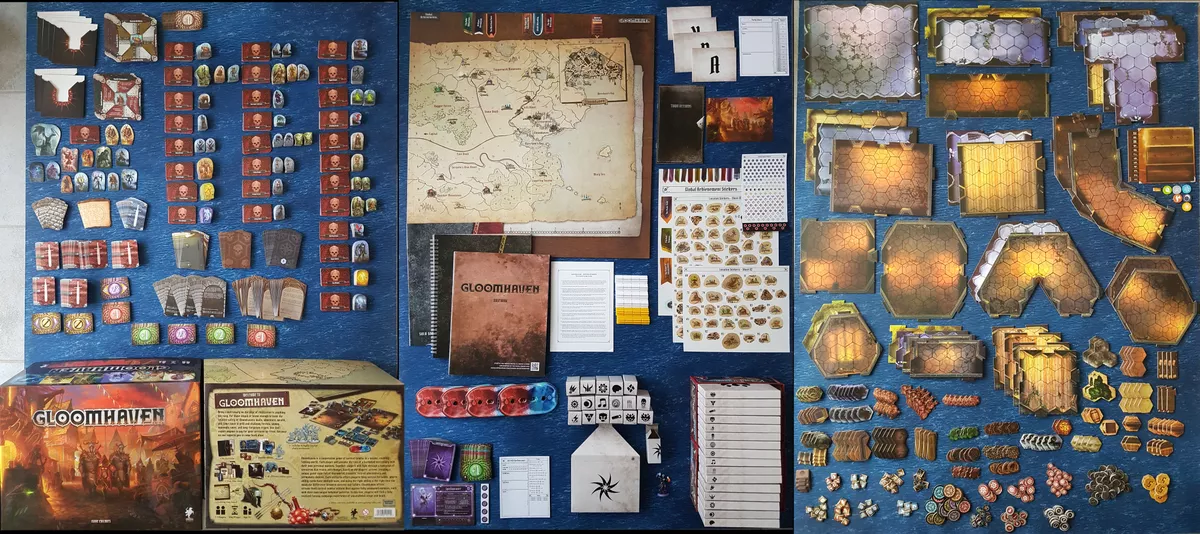
\includegraphics[width=0.9\textwidth]{resources/figures/gloomhaven.png}
    \caption{Fyzické komponenty deskové hry Gloomhaven.\cite{gloomhaven}}
    \label{fig:gloomhaven_contents}
\end{figure}

Fyzická součást hry obsahuje mapu světa, na kterou hráči postupně přilepují nálepky odemčených lokací a svých úspěchů. Hra obsahuje díly lokací, což jsou části hrací desky, které lze složit k sobě. Tyto části jsou potištěny hexagonovou sítí, která slouží jako políčka pro hráčské figurky. Dále se zde nachází kniha lokací, která popisuje příběh a udává rozložení a díly potřebné pro složení jednotlivých lokací. Každý typ nepřítele má svou kartu statistik a vlastní balíček karet, které určují jeho chování a možnosti. Dále je pak jeden společný balíček modifikátorů (karet, které namísto kostek slouží k vytváření nahodilých výsledků) pro všechny nepřátele. Podobně má každá postava také svůj balíček a kartu statistik, zároveň má však každý hráč vlastní balíček modifikátorů a počítadlo životů. Figurky postav jsou vyrobeny z plastu a jsou velice detailní. Kartonové figurky s plastovými stojánky představují nepřátele. Dále hra obsahuje velké množství kartiček předmětů, které hráči mohou používat, tokeny peněz, poškození a efektů.